\chapter{Specifikacija programske potpore}
		
	\section{Funkcionalni zahtjevi}
	
	\textbf{\textit{dio 1. revizije}}\\
	
	
	
	
	\noindent \textbf{Dionici:}
	
	\begin{packed_enum}
		
		\item Zaposlenici\begin{packed_enum}
			\item Revizor			
			\item Računovođa
			\item Normalan zaposlenik
		\end{packed_enum}
		
		\item Direktor
		\item Razvojni tim
		
		
	\end{packed_enum}
	
	\noindent \textbf{Aktori i njihovi funkcionalni zahtjevi:}
	
	
	\begin{packed_enum}
		\item  \underbar{Neregistrirani/neprijavljeni korisnik (inicijator) moze::}
		
		\begin{packed_enum}
			
			\item pristupiti Login aktivnosti
			\item pristupiti Sign-up aktivnosti
			
		\end{packed_enum}
		
		\item  \underbar{Radnik može:}
		
		\begin{packed_enum}
			
			\item pristupiti Login aktivnosti i prijaviti se
			\item skenirati dokument i podvrti točnost skeniranja ili označiti dokument kao krivo skeniran
			\item pogledati svoju povijest skeniranja
			
		\end{packed_enum}
		
		\item  \underbar{Računovođa može:}
		
		\begin{packed_enum}
			
			\item pristupiti Login aktivnosti i prijaviti se
			\item skenirati dokument i podvrti točnost skeniranja ili označiti dokument kao krivo skeniran
			\item pogledati svoju povijest skeniranja
			\item arhivirati dokument
			\item poslati dokument direktoru na potpis
			\item arhivirati potpisani dokument
			\item dobiti pregled dokumenta prije slanja na potpis / arhiviranja 
			
		\end{packed_enum}
		
		\item  \underbar{Revizor može:}
		
		\begin{packed_enum}
			
			\item pristupiti Login aktivnosti i prijaviti se
			\item skenirati dokument i podvrti točnost skeniranja ili označiti dokument kao krivo skeniran
			\item pogledati svoju povijest skeniranja
			\item provjeriti dokument i preusmijeriti ga računovođi koji je zadužen za taj tip dokumenta
			\item dobiti pregled dokumenta prije slanja na preusmjerivanja
			
			
			
		\end{packed_enum}
		
		\item  \underbar{Direktor može:}
		
		\begin{packed_enum}
			
			\item pristupiti Login aktivnosti i prijaviti se
			\item skenirati dokument i podvrti točnost skeniranja ili označiti dokument kao krivo skeniran
			\item pogledati svoju povijest skeniranja
			\item vidjeti statistike radnika firme
			\item potpisati dokument
			\item dobiti pregled dokumenta prije slanja na preusmjerivanja
			
		\end{packed_enum}
		\item  \underbar{Baza podataka:}
		
		\begin{packed_enum}
			
			\item pohranjuje sve podatke o korisnicima i njihovim ovlastima
			\item pohranjuje skenirane dokumente i ispavnost njihovog skeniranja
			
			
		\end{packed_enum}
		
		
	\end{packed_enum}
	
	\eject 
	
	
	
	\subsection{Obrasci uporabe}
	
	\textbf{\textit{dio 1. revizije}}
	
	\subsubsection{Opis obrazaca uporabe}

	
	
	\noindent \underbar{\textbf{UC1 - Login}}
	\begin{packed_item}
		
		\item \textbf{Glavni sudionik: }Korisnik aplikacije
		\item  \textbf{Cilj:} prijaviti se u aplikaciju
		\item  \textbf{Sudionici:} Baza podataka
		\item  \textbf{Preduvjet:} Korisnik je dobio password i username od direktora
		\item  \textbf{Opis osnovnog tijeka:}
		
		\item[] \begin{packed_enum}
			
			\item Korisnik aplikacije unosi username i password u to predviđena "text input-a"
			\item pritišće Login gumb
			\item biva preusmjeren na određenu aktivnost, ovisno o svojoj ulozi unatar firme
			
		\end{packed_enum}
		
		\item  \textbf{Opis mogućih odstupanja:}
		
		\item[] \begin{packed_item}
			
			\item[1.a] Unos krivih podataka
			\item[] \begin{packed_enum}
				
				\item Ponoviti unos, te paziti prilikom unosa podataka
				\item Provjeriti s direktorom ispravnost podataka
				
			\end{packed_enum}
			
			
		\end{packed_item}
	\end{packed_item}
	
	\noindent \underbar{\textbf{UC2 - Skreniranje dokumenta}}
	\begin{packed_item}
		
		\item \textbf{Glavni sudionik: }Korisnik aplikacije
		\item  \textbf{Cilj:} Skrenirati dokument
		\item  \textbf{Sudionici:} Baza podataka, Revizor
		\item  \textbf{Preduvjet:} Korisnik je prijavljen
		\item  \textbf{Opis osnovnog tijeka:}
		
		\item[] \begin{packed_enum}
			
			\item Korisnik aplikacije pritišće gumb za odabir skeniranja dokumenta
			\item Smiruje mobilni uređaj kako skeniranje ne bi bilo mutno
			\item Fokusira kameru
			\item Pritišće gumb za skeniranje, to jest slikanje dokumenta
			\item Korisnik odabire je li dokument ispravno skeniran
			\item Ako je dokument skreniran od strane zaposlenika i obilježen kao ispravno skeniran, taj dokument se šalje revizoru
			\item Ako revizor skenira dokument onda se dokument šalje računovođi koji je zadužen za tu vrstu dokumenta
			
			
		\end{packed_enum}
		
		\item  \textbf{Opis mogućih odstupanja:}
		
		\item[] \begin{packed_item}
			
			\item[2.a] Mutna slika
			\item[] \begin{packed_enum}
				
				\item Pokušati držati mobilni uređaj mirno pri skeniranju
				
				
			\end{packed_enum}
			
			\item[5.a] Neispravno skeniran dokoment
			\item[] \begin{packed_enum}
				
				\item Skenirati dokument ponovo
				
				
			\end{packed_enum}
			
			
		\end{packed_item}
	\end{packed_item}
	
	
	
	\noindent \underbar{\textbf{UC3 - Preusmjeravanje dokumenta računovođi}}
	\begin{packed_item}
		
		\item \textbf{Glavni sudionik: }Revizor
		\item  \textbf{Cilj:} Preusmjeriti podatke
		\item  \textbf{Sudionici:} Baza podataka, Računovođa
		\item  \textbf{Preduvjet:} Revizor je prijavljen i ima dokument koji može preusmjeriti
		\item  \textbf{Opis osnovnog tijeka:}
		
		\item[] \begin{packed_enum}
			
			\item Revizor pritišće gumb za 
			pregled "dobro" skeniranih dokumenata
			\item Potvrđuje da je dokument dobro skeniran pritiskom na taj dokument
			\item Odabirom ispravnog dokumenta može ga poslati računovođi koji je zadužen za taj dokument prtiskom gumba "pošalji računovođi" i odabirom računovođe
			
			
		\end{packed_enum}		
	\end{packed_item}
	
	
	
	\noindent \underbar{\textbf{UC4 - Arhiviranje dokumenta}}
	\begin{packed_item}
		
		\item \textbf{Glavni sudionik: }Računovođa
		\item  \textbf{Cilj:} Arhivirati ispravno skenirani dokument
		\item  \textbf{Sudionici:} Baza podataka
		\item  \textbf{Preduvjet:} Računovođa je prijavljen i ima dokument koji može arhivirati
		\item  \textbf{Opis osnovnog tijeka:}
		
		\item[] \begin{packed_enum}
			
			\item Računovođa pritišće gumb za 
			pregled potencijalno potpisanih i preusmjerenih dokumenata
			\item Računovođa pritiskom na dokument označuje dokument za arhiviranje ili slanje na potpis
			\item Utvrđuje da je dokument ispravno preusmjeren ili potpisan, te pritišće gumb "Arhiviraj"
			\item Dokumentu dobiva oznaku "arhiviran" u bazi podataka
			
			
			
		\end{packed_enum}		
	\end{packed_item}
	
	\noindent \underbar{\textbf{UC5 - Slanje dokumenta direktoru na potpis}}
	\begin{packed_item}
		
		\item \textbf{Glavni sudionik: }Računovođa
		\item  \textbf{Cilj:} Poslati dokument direktoru na potpis
		\item  \textbf{Sudionici:} Baza podataka, direktor
		\item  \textbf{Preduvjet:} Računovođa je prijavljen i ima dokument koji može poslati direktoru
		\item  \textbf{Opis osnovnog tijeka:}
		
		\item[] \begin{packed_enum}
			
			\item Računovođa pritišće gumb za 
			pregled potencijalno potpisanih i preusmjerenih dokumenata
			\item Računovođa odabire ne-potpisan dokument i šalje ga direktoru na potpis pritiskom gumba "pošalji na potpis"
			
			
			
		\end{packed_enum}		
	\end{packed_item}
	
	\noindent \underbar{\textbf{UC6 - Potpis dokumenta}}
	\begin{packed_item}
		
		\item \textbf{Glavni sudionik: }Direktor
		\item  \textbf{Cilj:} Potpisati dokument
		\item  \textbf{Sudionici:} Baza podataka
		\item  \textbf{Preduvjet:} Direktor je prijavljen i ima dokument koji može potpisati
		\item  \textbf{Opis osnovnog tijeka:}
		
		\item[] \begin{packed_enum}
			
			\item Direktor pritišće gumb "Dokumenti za potpis" za 
			pregled preusmjerenih dokumenata
			\item Direktor odabire jedan ili više ne-potpisanih dokumenta i potpisuje ih pritiskom gumba "Potpiši"
			\item Dokument se sprema u bazu podataka kao potpisan dokument
			
			
		\end{packed_enum}		
	\end{packed_item}
	
	\noindent \underbar{\textbf{UC7 - Pregled povijesti dokumenata}}
	\begin{packed_item}
		
		\item \textbf{Glavni sudionik: }Direktor
		\item  \textbf{Cilj:} Pregledati povijest dokumenata
		\item  \textbf{Sudionici:} Baza podataka, direktor
		\item  \textbf{Preduvjet:} Direktor je prijavljen i baza podataka ima barem jedan dokument
		\item  \textbf{Opis osnovnog tijeka:}
		
		\item[] \begin{packed_enum}
			
			\item Direktor pritišće gumb za 
			pregled povijest i statisiku
			\item Direktor pritišće gumb za pregled skeniranih dokumenata
			
			
		\end{packed_enum}		
	\end{packed_item}
	
	\noindent \underbar{\textbf{UC8 - Pregled statistike  zaposlenika}}
	\begin{packed_item}
		
		\item \textbf{Glavni sudionik: }Direktor
		\item  \textbf{Cilj:} Pregledati statistike zaposlenika
		\item  \textbf{Sudionici:} Baza podataka, direktor
		\item  \textbf{Preduvjet:} Direktor je prijavljen i postoji barem jedan zaposlenik
		\item  \textbf{Opis osnovnog tijeka:}
		
		\item[] \begin{packed_enum}
			
			\item Direktor pritišće gumb za 
			pregled povijest i statisiku
			\item Direktor pritišće gumb za pregled statistike radnika
			
			
			
			
		\end{packed_enum}	
		\item  \textbf{Opis mogućih odstupanja:}
		
		\item[] \begin{packed_item}
			
			\item[2.a] Ne-prikaz nekih statistika
			\item[] \begin{packed_enum}
				
				\item Ako se neke statistike ne prikažu, to znači da korisnik nema ovlasti za te radnje
			\end{packed_enum}	
		\end{packed_item}
	\end{packed_item}
	
	
	
	\noindent \underbar{\textbf{UC9 - Stvaranje korisnika}}
	\begin{packed_item}
		
		\item \textbf{Glavni sudionik: }Direktor
		\item  \textbf{Cilj:} Stvoriti korisnika
		\item  \textbf{Sudionici:} Baza podataka, korsinik
		\item  \textbf{Preduvjet:} Direktor je prijavljen
		\item  \textbf{Opis osnovnog tijeka:}
		
		\item[] \begin{packed_enum}
			
			\item Korisnik pritišće gumb "sign up" za 
			Signup aktivnost
			\item Korisnik upisuje podatke na za to predviđena mjesta
			\item Korisnik pritišće gumb "Signup"
			\item Korisnik biva pohranjen u bazu podataka
			
			
		\end{packed_enum}		
	\end{packed_item}
				
					
				\subsubsection{Dijagrami obrazaca uporabe}
					
				
					
				
			\subsection{Sekvencijski dijagrami}
			\subsubsection{Login korisnika}
			
			Korisnik unosi korisničko ime i lozinku te se pokušava ulogirati u aplikaciju. Uneseni podaci se preko API Gatewaya i lambda funkcije šalju u bazu podataka. Tamo se provjerava postoji li korisnik s unesenim korisničkim imenom, ako ne postoji korisniku su ispisuje poruka LoginInvalid. Ako je baza pronašla korisnika provjerava njegovu šifru u bazi podataka s upisanom šifrom i ako se one podudaraju ispisuje korisniku LoginValid, u suprotnom ispisuje LoginInvalid.
			\eject
			
			\begin{figure}
				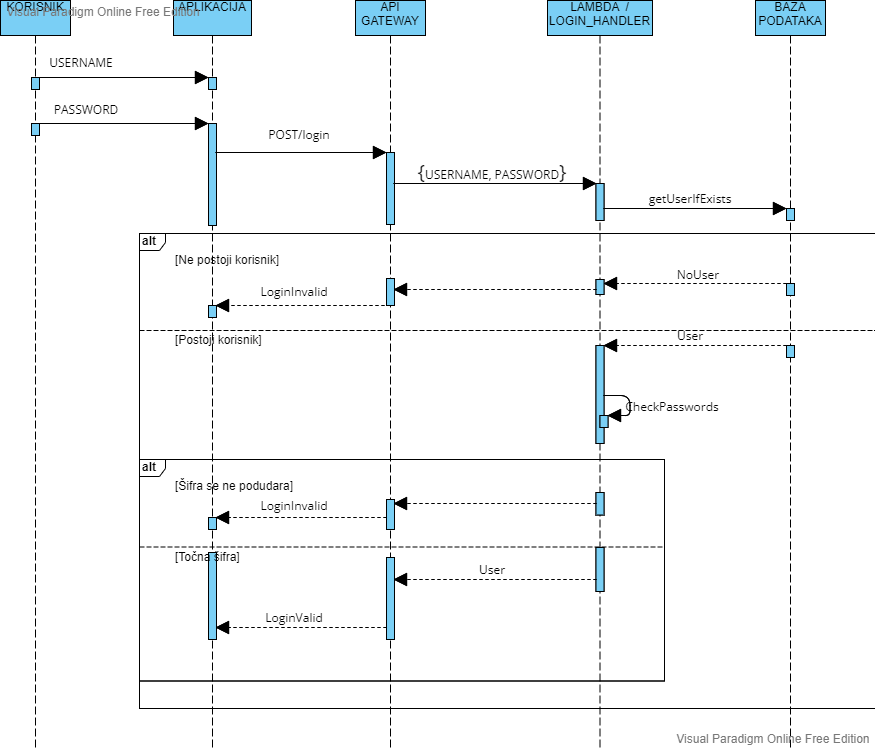
\includegraphics[width=\linewidth]{./dijagrami/Login.png}
				\caption{Sekvencijski dijagram za login}
				\label{fig:Login}
			\end{figure}
			
			
			
			\subsubsection{Registracija korisnika}
			
			Korisnik unosi korisničko ime, ime, prezime, lozinku i poziciju. Uneseni se podaci preko API Gatewaya i lambda funkcije šalju u bazu podataka. Tamo se provjerava postoji li već korisnik s navedenim korisničkim imenom, ako da ispisuje LoginInvalid. U suprotnom slučaju unosi korisnika u bazu podataka i ispisuje LoginValid.
			\eject
			
			\begin{figure}
				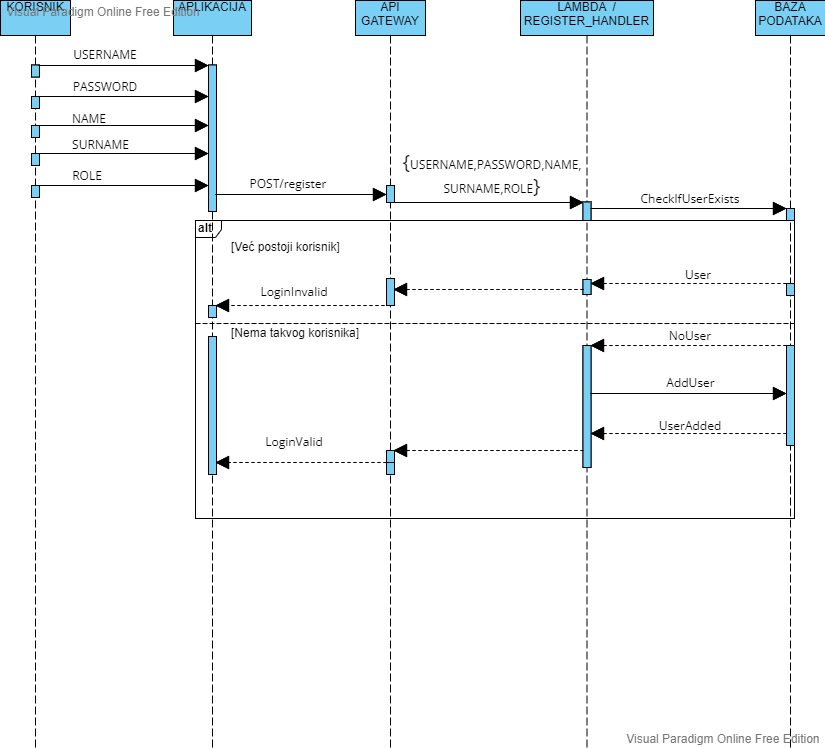
\includegraphics[width=\linewidth]{./dijagrami/Register.png}
				\caption{Sekvencijski dijagram za registraciju}
				\label{fig:Register}
			\end{figure}
			\subsubsection{OCR funkcija}
			
			Korisnik skenira željeni dokument te u aplikaciji poziva funkciju OCR koja mu vraća sažetak dokumenta. Zatim korisnik odlučuje točnost dokumenta te to označi u aplikaciji. Sažetak dokumenta i točnost se šalju u bazu podataka neovisno o korisnikovom odabiru.
			\eject
			
			\begin{figure}
				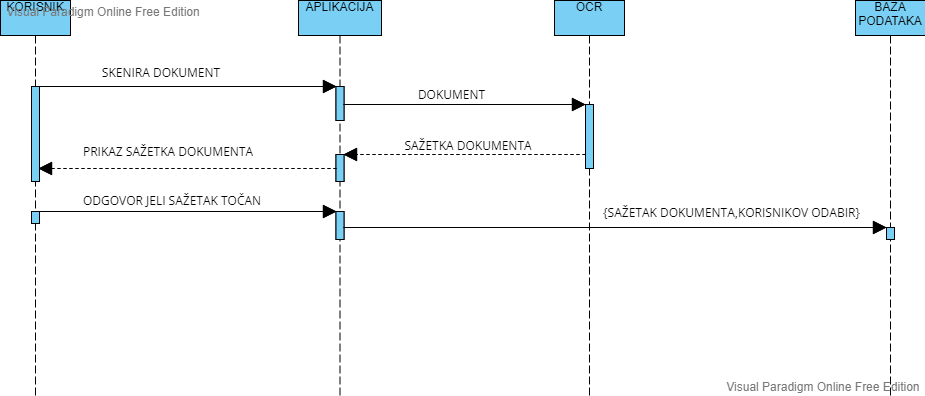
\includegraphics[width=\linewidth]{./dijagrami/OCR.png}
				\caption{OCR funkcija}
				\label{fig:OCR}
			\end{figure}
			
			\subsubsection{Povijest svih skeniranih dokumenata zaposlenika}
			
			Zaposlenik u aplikaciji traži povijest svih svojih skeniranih dokumenata. Preko API Gatewaya i lambda funkcije u bazi podatak se provjerava postoji li uopće neki skenirani dokument od zaposlenika, ako ne ispisuje zaposleniku da je povijest skeniranja prazna. Ako već postoje skenirani dokumenti u bazi podataka, aplikacija ih daje na pregled zaposleniku.
			\eject
			
			\begin{figure}
				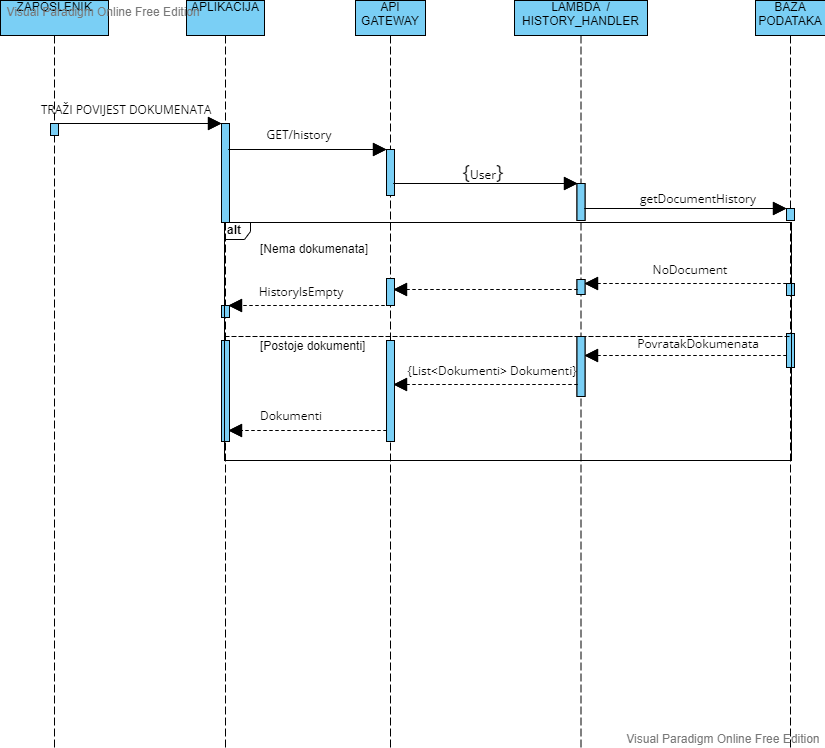
\includegraphics[width=\linewidth]{./dijagrami/History.png}
				\caption{Povijest svih skeniranih dokumenata zaposlenika}
				\label{fig:History}
			\end{figure}
			
		\section{Ostali zahtjevi}
		
			\textbf{\textit{dio 1. revizije}}\\
		 
			 
			 Podržani jezik našeg programskog sučelja je Engleski. Vrijeme odziva\\ aplikacije je gotovo trenutačno, možda oko pola sekunde čekanja između klika na login i ulaska u aplikaciju. Podržani broj korisnika nema gornje ograničenje, zato što uvijek možemo dodatno skalirati sustav. Trenutno koristimo AWS free tier usluge te imamo 20GB alociranog prostora i milijun besplatnih zahtjeva na AWS lambdu mjesečno. Sa rastom broja korisnika možemo po potrebi skalirati sustav po cijeni ponuđenoj od strane AWS-a. Podržana mobilna platforma je Android OS, aplikacija je pisana u Javi (Android Studiu) i Pythonu. Razina zaštite na\\ kompletnom sustavu je relativno niska, u bazu podataka se upisuje lozinka u\\ izvornom obliku, bez bilo kakve vrste kriptiranja. Jedina zaštita koju imamo je to što AWS, na kojem nam se sve nalazi, koristi https protokol. Aplikacija je jako pouzdana što se tiče registiranja korisnika i zapisa njihovih podataka u bazu podataka na AWS RDS poslužitelju te dohvaćanju tih podataka iz baze i validaciji prilikom prijave. Registracija je lagana i jednostavna, klikom na "\textit{signup}" gumb se mogu unijeti svi potrebni podaci, a korisničko ime i lozinka su kasnije potrebni za prijavu u sustav.
			 Korištenje aplikacije nakon prijave je isto jako jednostavno, sve opcije za svakog korisnika su ponuđene odmah na početnoj stranici aplikacije.
			 
			 
			 
	